\documentclass[../skript.tex]{subfiles}

% Use standard labeling

The lecture will be split in 3 chapters:
\begin{enumerate}
	\item [Chapter $I$] Basic notions of continuous mechanics
	\item [Chapter $II$] PDE techniques for fluid mechanics
	\item [Chapter $III$] Solid mechanics $\to$ Calculus of variations
\end{enumerate}

\chapter{Basic notions of continuous mechanics}\label{c1}
	\section{Modelling a physical system}\label{c1se1}
		Point $\to$ continuous mechanics\par 
		Regarding the modelling we have 2 main examples:\par
		\textbf{a)} Flow of a fluid around an obstacle (stone, airplane), or in a pipe 
		\begin{figure}[ht]
		\centering
		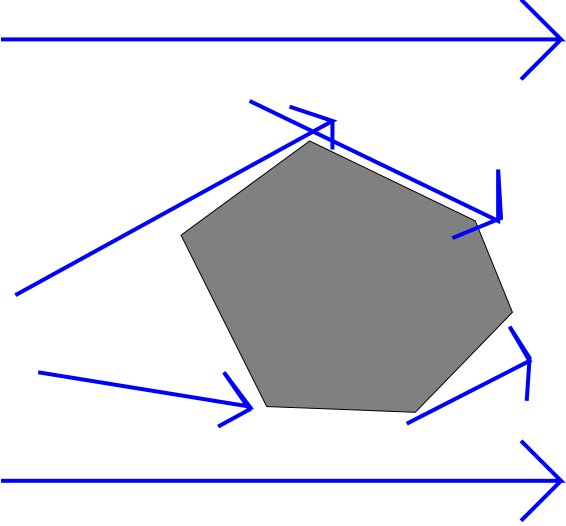
\includegraphics[width=0.2\textwidth]{Images/pde2.png}
		\caption{Fluid flows around an obstacle}
		\end{figure}
		\par 
		\textbf{b)} Deformations in a solid (ex. a sponge)\par 
		\begin{figure}[ht]
		\centering
		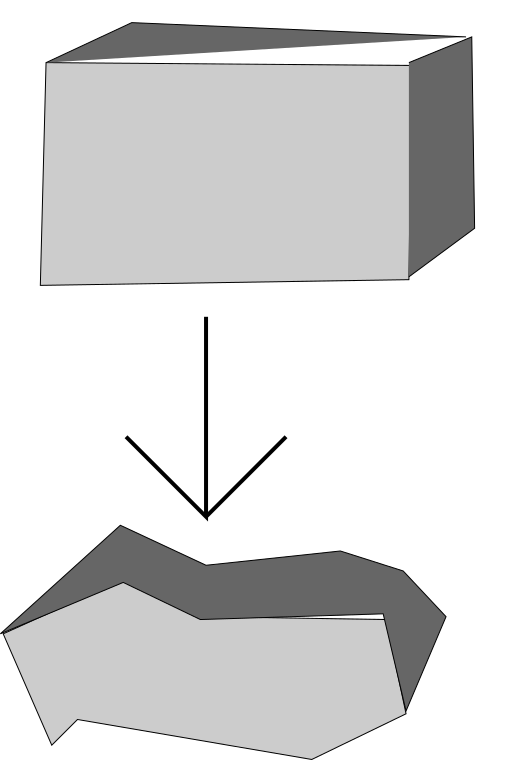
\includegraphics[width=0.2\textwidth]{Images/pde1.png} 
		\caption{Deformation of a sponge}
		\end{figure}
		\subsection*{Physical description}
			\textbf{Microscropic:} atosm/molecules,  $\sim 10^{26}$ molecules $\Rightarrow$ This is hard!!!\newline\noindent
			\textbf{Macroscopic:} $\Rightarrow$ See water / sponge as continuous materials! This leads to the concept of continuous mass distribution (has to be defined).\par
			In general, Physics leads to PDE, this means we get a PDE if we translate a physical problem into mathematics.
			\subsubsection*{From physics to PDE}
			\begin{enumerate}
				\item Identify the mathematical object (what is the size of interest (temperature, pressure, dislocation, ...)? ) $\Rightarrow$ This yields a function $u(\vec x,t)$, for $\vec x\in \mathbb{R}^3,\,t>0$ and $u\in\mathbb{R}^n$
				\item Use physical laws and some assumptions on the material $\Rightarrow$ This shows that the size of interest needs to satisfy a (system of) PDE
				\item Boundary conditions tell us, how the sample (domain) interacts with the external world
				\item Set initial conditions for the object of interest, i.e. specify $u(\vec x,0)$
			\end{enumerate}

			\begin{example}
				Consider a fluid flowing around an obstacle.
				\begin{enumerate}
					\item $\vec u(\vec x,t)$ is the velocity of a small portion of fluid near $\vec x$ at time $t$. The domain $K$ is compact in $\mathbb{R}^3$, so we look for 
					\begin{IEEEeqnarray*}{rCl}
						u:&\mathbb{R}^3\setminus K \times (0,\infty) &\to\mathbb{R}^3\\
						&(x,t)&\mapsto \vec u(x,t) 
					\end{IEEEeqnarray*}

					\item Use physical laws (conservation laws). Make assumptions on the fluid, i.e. compressible / incompressible. This gives us different PDE.\newline\noindent
					In the incompressible case $\Rightarrow$ \textbf{Navier Stokes equations}
					\begin{IEEEeqnarray*}{rCl}
						\varrho_0 [ \partial_t\vec u + (\vec u\cdot\vec\nabla)\vec u] &=& -\vec\nabla p + \eta \Delta\vec u\\
						\dive\vec u &=& 0
					\end{IEEEeqnarray*}
					for $x\in\mathbb{R}^3\setminus K, t>0$. Here we used
					\begin{itemize}
						\item the mass density $\varrho_0 > 0$ 
						\item the dynamical viscosity $\eta > 0$
						\item the pressure $p:\mathbb{R}^3\setminus K\times \mathbb{R}_+\to\mathbb{R}$
						\item and the notation
						\[
							\vec u\cdot\vec\nabla = \sum_{j=1}^3 u_j \frac{\partial}{\partial u_j}
						\]
						so
						\[
							[(\vec u\cdot\vec\nabla)\vec u]_i = \left[ \sum_{j=1}^3 u_j\frac{\partial}{\partial u_j} \right] u_i,
						\]
						as well as 
						\[
							(\vec\nabla p)_i = \frac{\partial}{\partial u_i}p
						\]
						and
						\[
							[\Delta\vec u]_i = \left[ \sum_{j=1}^3 \left(\frac{\partial}{\partial u_j}\right)^2 \right]u_i
						\]
					\end{itemize}
					\item  Impose boundary conditions. We have 2 possible boundaries: either $\partial K$ or the behaviour of our size at interest at infinite distance.\newline\noindent
					For $\partial K$ we have \underline{two} types of possible boundary conditions:
					\begin{itemize}
						\item Dirichlet B.C. fix the value of our size of interest at $\partial K$, i.e. fix $u_{|\partial K}$. The homogeneous B.C. $u_{|\partial K}$ is also called no slip (sticky) boundary condition
						\item Neumann B.C. fix $(\nabla_N u)_{|\partial K}$, i.e. the gradient in outer normal direction of $\partial K$. This fixes not the specific value of the size of interest, but its amount of change (that is the gradient)
					\end{itemize}
					At infinity we do the following: If there is no $K$, we assume that the fluid flows at constant speed (it does not hit any obstacle), i.e. $\vec u(x,t) = \vec u_\infty$ is constant.
					\item Impose initial conditions: Give $u(x,0) = \vec u_0(x)$, where $\vec u_0$ is a fixed velocity distribution.
				\end{enumerate}
			\end{example}
			\subsubsection*{From PDE to physics}
				\begin{itemize}
					\item [a)] Which PDE are physically reasonable? This leads to \emph{dimensional analysis}.
					\item [b)] Usually one experiments on a small sized sample (small toy airplane) in order to get a describing PDE. Does this PDE also describe the life-size system (true airplane)? This leads to the \emph{similarity principle}.
				\end{itemize}
				\textbf{a) Dimensional Analysis}\par  We cannot compare meters and seconds! All terms in a PDE must have the same dimension! We have the following basic dimensions:
				\begin{itemize}
					\item [L] length
					\item [T] time
					\item [M] mass
				\end{itemize}
				Thus e.g. the dimension of the velocity is 
				\[
					[u] = \frac{L}{T}.
				\]
				Consider the Navier Stokes equation: 
				\[
					-\nabla p + \eta \Delta u = \varrho_0\partial_t u + \varrho_0(u\cdot\nabla)u
				\]
				For dimensional analysis we need to check the dimension of each of the occuring terms:
				\begin{itemize}
					\item $[u] = \frac{L}{T}$
					\item $[p] = \frac{[\text{force}]}{[\text{area}]}$ and $[\text{area}] = L^2$
					\item $[\text{force}] = ?$ ? Newtons law tells us $F=ma$ so 
					\[
						[F] = M\frac{L}{T^2}
					\]
					Thus  $[p] = \frac{ML}{T^2}\frac{1}{L^2} = \frac{M}{T^2 L}$
					\item $[\nabla p] = [\frac{\partial}{\partial u_i}p] = \frac{[p]}{L} = \frac{M}{T^2L^2}$
					\item $[\varrho_0\partial_t u] = ?$ ? We have 
					\[
						[\partial_t u] = \frac{[u]}{T} = \frac{L}{T^2}
					\]
					and
					\[
						\varrho_0 = \frac{\text{mass}}{\text{volume}}\quad\Rightarrow\quad[\varrho_0] = \frac{M}{L^3}
					\]
					thus
					\[
						[\varrho_0\partial_t u] = \frac{M}{L^3}\frac{L}{T^2} = \frac{M}{L^2T^2}
					\]
					\item $[(u\nabla)u] = \frac{[u]^2}{L} = \frac{L^2}{T^2}\frac{1}{L} = \frac{L}{T^2}$. We can do the first step as $u$ appears twice on the LHS, so its dimension enters quadratically
					\item $[\eta\Delta u] \overset!=\frac{M}{T^2L^2}$ has to hold. We have
					\[
						[\eta]\underbrace{[\Delta u]}_{=\frac{u}{L^2}} = \frac{M}{L^2T^2}
					\]
					and
					\[
						[\eta] \cdot \frac{L}{\cancel{T}}\frac{1}{\cancel{L^2}} = \frac{M}{\cancel{T^2}\cancel{L^2}}.
					\]
					We will see later that $[\eta] = \frac{M}{LT}$ really holds.
				\end{itemize}

				\textbf{b) Similarity principle}\par 
				Geometrically 2 triangles are similar if their \emph{adimensional} parameter coincide.
				\begin{figure}[ht]
					\centering
					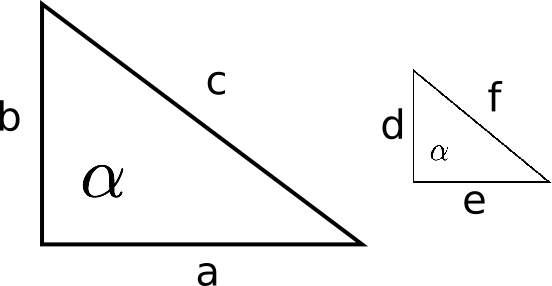
\includegraphics[width=0.6\textwidth]{Images/pde3.png}
					\caption{The triangles are similar, as $\sin \alpha = \frac{b}{a} = \frac{d}{e}$, so the adimensional parameters coincide}
					\label{fig3}
				\end{figure}
				Analogeously to the case of triangles (see \cref{fig3}) two physical processes are similar if the corresponding adimensional patrameters of the processes coincide. This means we need first to identify the adimensional parameters and then write the PDE in a dimensionless form (this can be done for physical systems that are similar!)\par 

				\begin{example}
					Consider again the case of Navier-Stokes:
					\[
						-\nabla p + \eta\Delta u = \varrho_0\partial_tu + \varrho_0(u\cdot\nabla)u
					\]
					with the variables $x,t$. Define new variables 
					\begin{eqnarray*}
						y &\coloneqq& \frac{x}{x_0}\\
						\tau &\coloneqq& \frac{t}{t_0}
					\end{eqnarray*}
					with $[x_0] = L,\,[t_0] = T$. A natural choice for $x_0$ is $x_0 = \diam K$ s.t. near the obstacle we have $|y|\approx 1$ and $|y| >>1$ far away from the obstacle. Unfortunately there is no natural choice for $t_0$. We have
					\begin{eqnarray*}
						\tilde u(\tau,y) &=& u(t(\tau),x(y))\\
						\tilde p(\tau,y) &=& p(t(\tau),x(y))
					\end{eqnarray*}
					thus we get
					\[
						\partial_t u(t,x) = \partial_t\tilde u(\tau(t),y(x)) = \partial_\tau\tilde u\cdot\frac{\partial\tau}{\partial t}
					\]
					and
					\[
						\frac{\partial}{\partial u_i}u = \sum_j \frac{\partial \tilde u}{\partial y_j}\frac{\partial y_j}{\partial u_i} = \left(\frac{\partial\tilde u}{\partial y_i}\right)\frac{1}{x_0}.
					\]
					Then, $\tilde u,\tilde p$ satisfy
					\[
						-\frac{1}{x_0} \nabla_y\tilde p + \eta\frac{1}{x_0^2}\Delta_y\tilde u = \varrho_0\left[ \frac{1}{t_0}\partial_\tau\tilde u + \frac{1}{x_0}\left( \vec{\tilde u}\cdot\vec\nabla y \right) \tilde u\right]
					\]
					but $\tilde p,\tilde u$ still have a dimension. Define
					\begin{IEEEeqnarray*}{rCl}
						\tilde v(\tau,y) &\coloneqq& \frac{\tilde u(\tau,y)}{u_0}\\
						q(\tau,y) &\coloneqq& \frac{\tilde p(\tau,y)}{p_0}
					\end{IEEEeqnarray*}
					using $u_0 > 0$ with $[u_0] = [\text{velocity}]$ and $p_0>0$ with $[p_0] = [\text{pressure}]$. How can we choose $u_0$ and $p_0$? A natural choice for $u_0$ would be $u_0 = |\vec u_\infty$ (where $\lim_{|x|\to\infty}u(x,t) = \vec u_\infty$ is a constant vector). Then
					\[
						v = \frac{\tilde u}{v_0} \quad\Rightarrow\quad |v| \overset{|y|\to\infty}\to \frac{1}.
					\]
					For $p_0$ there is no natural choice.\newline\noindent
					Replace in the PDE:
					\[
						-\frac{p_0}{x_0}\underbrace{\vec\nabla q}_{\text{adim.}} + \frac{u_0\eta}{x_0^2}\underbrace{\Delta v}_{\text{adim.}} = \frac{\varrho_0u_0}{t_0}\underbrace{\partial_t v}_{\text{adim.}} + \frac{\varrho_0^2}{x_0}\underbrace{(\vec v\cdot\vec\nabla)\vec v}_{\text{adim.}}
					\]
					Divide now by $\frac{\varrho_0v_0}{t_0}$:
					\[
						\partial_t v + \underbrace{\frac{v_0t_0}{x_0}}_{\text{adim.}} (v\nabla)v = \underbrace{-\frac{\varrho_0}{x_0}\frac{t_0}{\varrho_0v_0}}_{\text{adim.}}\nabla q + \underbrace{\frac{\eta}{x_0^2}\frac{t_0}{\varrho_0}}_{\text{adim.}}\nabla v
					\]
					Now we have 
					\begin{itemize}
						\item fixed $v_0,x_0$
						\item free $t_0,p_0$
						\item $\varrho_0,\eta$ given by the physical system
					\end{itemize}
					and we want to choose $t_0$ s.t. $\frac{v_0t_0}{x_0} = L = v_0 = \frac{x_0}{t_0}$, so
					\[
						\Rightarrow \frac{p_0t_0}{x_0\varrho_0v_0} = \frac{p_0}{\varrho_0v_0^2}.
					\]
					Choose $p_0$ s.t. $\frac{p_0}{\varrho_0 v_0^2} = 1$ so $p_0 = \varrho_0v_0^2$. Then
					\[
						\frac{\eta t_0}{x_0^2\varrho_0} = \frac{\eta}{\varrho_0v_0x_0} = \frac{1}{Re}
					\]
					where $Re$ is the so called \emph{Reynolds number}.
					In the end we get
					\begin{equation}
						\begin{aligned}
							\partial_\tau v + (v\cdot\nabla)v &=& -\nabla q + \frac{1}{Re}\Delta v\\
							\dive v &=& 0\\
							v(\tau,y)&\overset{\|y\|\to\infty}\longrightarrow& \frac{\vec u_\infty}{u_0}.
						\end{aligned}
					\end{equation}
					The reynolds number is the only term that contains information on the physical system!
				\end{example}

